\documentclass{report}

\usepackage{natbib}
\setcitestyle{authoryear,round}
\usepackage{graphics}
\usepackage{amsmath}
\usepackage{indentfirst}
\usepackage{hanging}
\usepackage[utf8]{inputenc}
\usepackage{hyperref}
\usepackage{amsmath}

\DeclareGraphicsExtensions{.pdf,.jpg}

% \VignetteIndexEntry{Create virtual species with sdmvspecies}
% \VignetteKeyword{species distribution modelling}
% \VignetteKeyword{virtual species}
% \VignetteDepends{ggplot2,grid}

\newcommand{\super}[1]{\ensuremath{^{\textrm{#1}}}}
\newcommand{\sub}[1]{\ensuremath{_{\textrm{#1}}}}
\newcommand{\R}{{\normalfont\textsf{R }}{}}







\usepackage{Sweave}
\begin{document}
\Sconcordance{concordance:sdmvspecies.tex:/home/howl/Documents/private/sdmvspecies/sdmvspecies/vignettes/sdmvspecies.Rnw:%
1 26 1 1 6 2 1 1 0 32 1 1 2 1 0 6 1 11 0 4 1 4 0 1 2 %
7 1 1 31 1 3 2 1 1 21 1 3 2 1 1 21 1 3 1 1 1 28 1 2 1 %
28 1 2 9 1 1 8 10 0 1 2 6 1 1 3 2 0 1 1 1 2 1 0 1 2 6 %
0 1 2 1 0 1 2 6 0 1 2 1 0 1 1 1 2 1 0 1 2 1 0 1 2 5 0 %
1 2 6 1 1 3 2 0 1 2 1 0 1 2 6 0 1 2 1 0 1 2 6 0 1 2 1 %
0 1 1 1 2 1 0 1 2 1 0 1 2 5 0 1 2 3 1 1 3 2 0 1 2 1 0 %
1 2 6 0 1 2 1 0 1 2 6 0 1 2 1 0 1 1 1 2 1 0 1 2 1 0 1 %
2 1 0 1 2 1 0 1 2 1 0 1 2 5 0 1 2 6 1}



\title{Create virtual species with sdmvspecies}
\author{Xiaoquan Kong}
\maketitle

% \tableofcontents
\chapter{Introduction}
Simulations of virtual species are more and more pupulation in testing the effects of different aspects of modellling and sampling strategy on performance fo species distribuiton models (SDMs).
This vignette illustrates how to create virtual species using sdmvspecies.
If you are using a recent version of \R, you can install SDMvspecies with this:

\texttt{install.packages("sdmvspecies")}

This work still progress, Suggestions are welcomed.

\chapter{Select a method}
There are many method which can create virtual species. Choice one that you think is suitable for your study.
\section*{Niche synthese method}
This method bases on paper "Assessing habitat-suitability models with a virtual species" \citep{hirzel_assessing_2001}.
In this method, the virtual species is generated by creating a simulated ecological niche in an multi-dimensional space,
for $i$ th-dimensional space, the ecological niche is calculate as $W_i$ * $H_i$, $W_i$ is the weight of this space and the $H_i$ is the virtual species's niche
suitability index (H $\epsilon$ [0,1]). The finally total niche suitability index is built as summarised in:
\[
H = \frac{1}{\sum_{i=1}^n W_i} \sum_{i=1}^n H_i W_i
\]
Which $H$ is the niche suitability of that cell, $H_i$ is the value of the $i$ th partial niche coefficient and the $W_i$ is weight of this partial niche suitability.
Habitat suitability is composed of many weighted average of partial niche suitability ($H_i$). Partial niche suitability ($H_i$) is project from environment by a function. We call this type of function "Niche resposne function", and it projects environment variable to niche suitability.
There are five kinds of "Niche response function", and we will explain them latter.
Let's do a simple example:

\begin{Schunk}
\begin{Sinput}
> library("sdmvspecies")
> library("raster")
> package.dir <- system.file(package="sdmvspecies")
> env.dir <- paste(package.dir, "/external/env", sep="")
> files <- list.files(path=env.dir, pattern="*.bil$", full.names=TRUE)
> env.stack <- stack(files)
> print(files)
\end{Sinput}
\begin{Soutput}
[1] "/home/howl/R/x86_64-pc-linux-gnu-library/3.2/sdmvspecies/external/env/bio1.bil" 
[2] "/home/howl/R/x86_64-pc-linux-gnu-library/3.2/sdmvspecies/external/env/bio11.bil"
[3] "/home/howl/R/x86_64-pc-linux-gnu-library/3.2/sdmvspecies/external/env/bio12.bil"
[4] "/home/howl/R/x86_64-pc-linux-gnu-library/3.2/sdmvspecies/external/env/bio14.bil"
[5] "/home/howl/R/x86_64-pc-linux-gnu-library/3.2/sdmvspecies/external/env/bio16.bil"
[6] "/home/howl/R/x86_64-pc-linux-gnu-library/3.2/sdmvspecies/external/env/bio5.bil" 
[7] "/home/howl/R/x86_64-pc-linux-gnu-library/3.2/sdmvspecies/external/env/bio7.bil" 
\end{Soutput}
\begin{Sinput}
> config <- list(c("bio1","1",2), c("bio12", "2", 2), c("bio5", "3", 1), c("bio7", "4", 2))
> species.raster <- nicheSynthese(env.stack, config)
> species.raster <- rescale(species.raster)
> plot(species.raster>0.7)
\end{Sinput}
\end{Schunk}
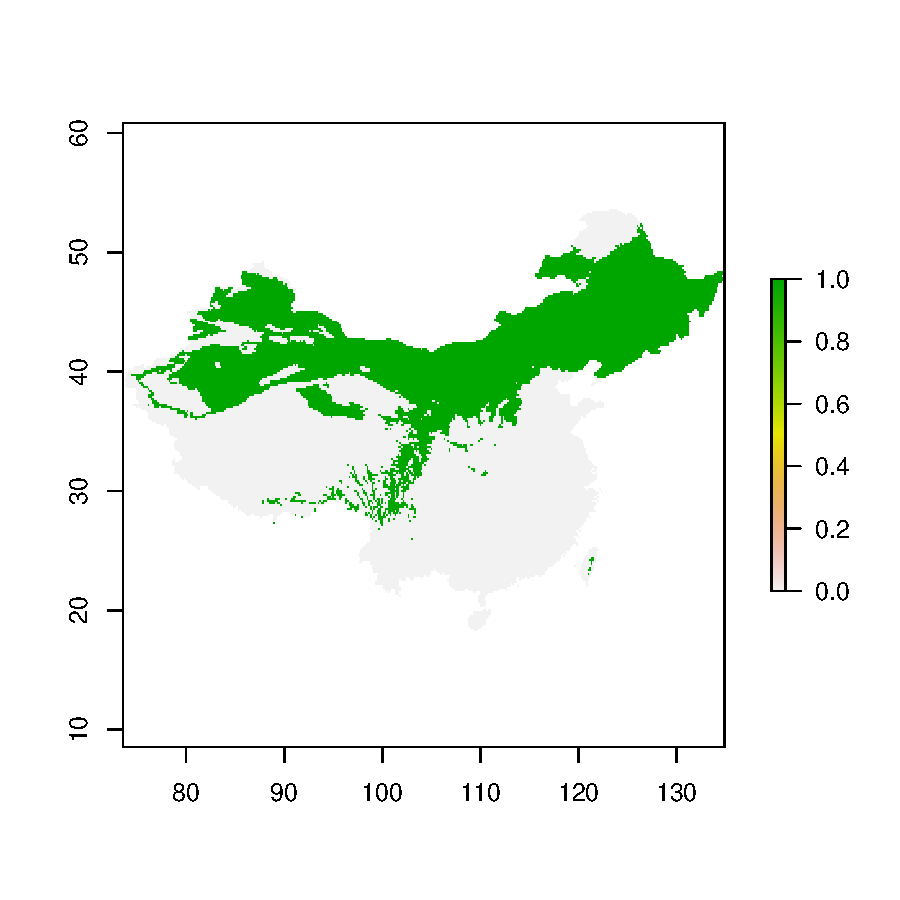
\includegraphics{sdmvspecies-niche_Synthsis_Method}

\subsection*{Configure response function}
The hardest part of this method is the config. Here we explain that,
in this method. You need configure a function: how the the species habit suitability index
response the environment variable. There are serveral response function currently that you can used:

\subsubsection*{Bell-shaped function}
In this method, species habit suitablity are bell-shaped function, see Figure:
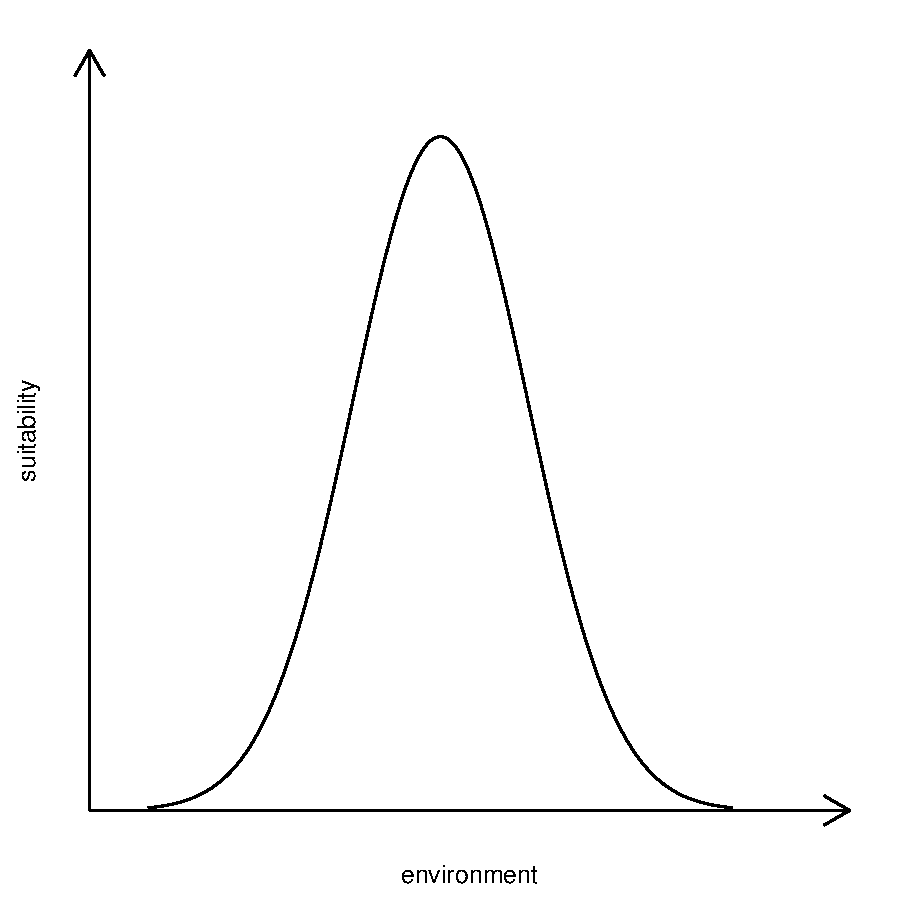
\includegraphics{sdmvspecies-bell_shaped_response_function}

\subsubsection*{Linear increase function}
In this method, species habit suitability are increas with the environment varability.
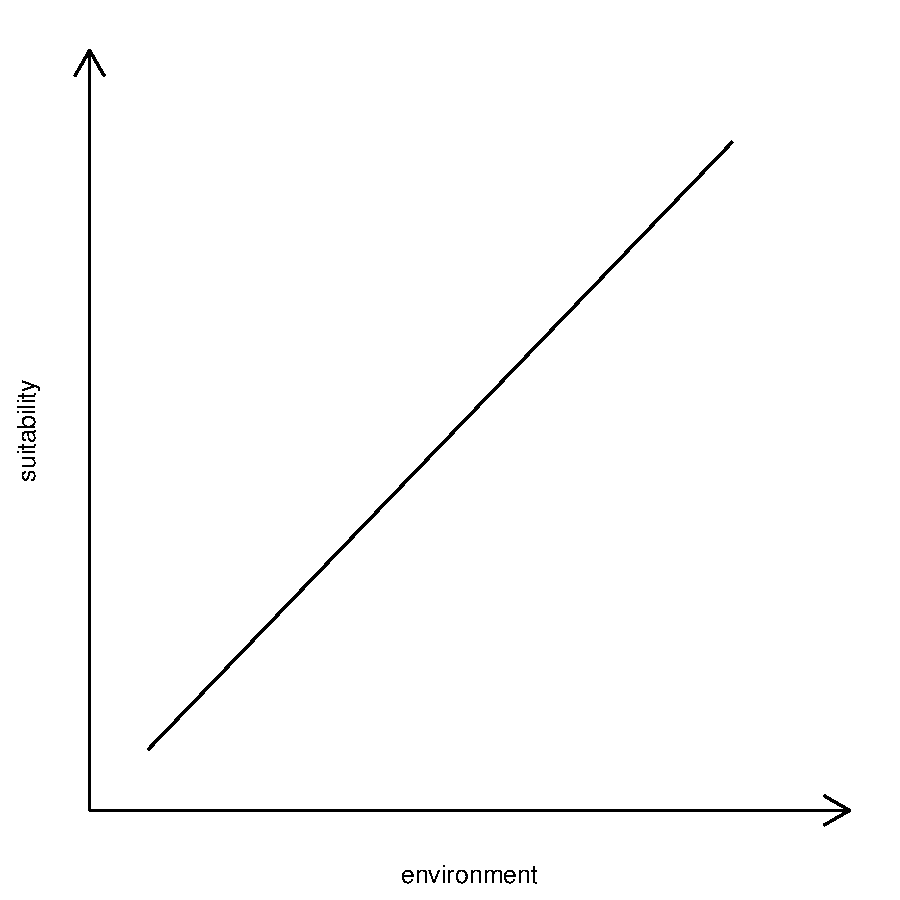
\includegraphics{sdmvspecies-linear_increasing_function}

\subsubsection*{Linear decrease function}
In this method, species habit suitability are decrease with the environment variably.
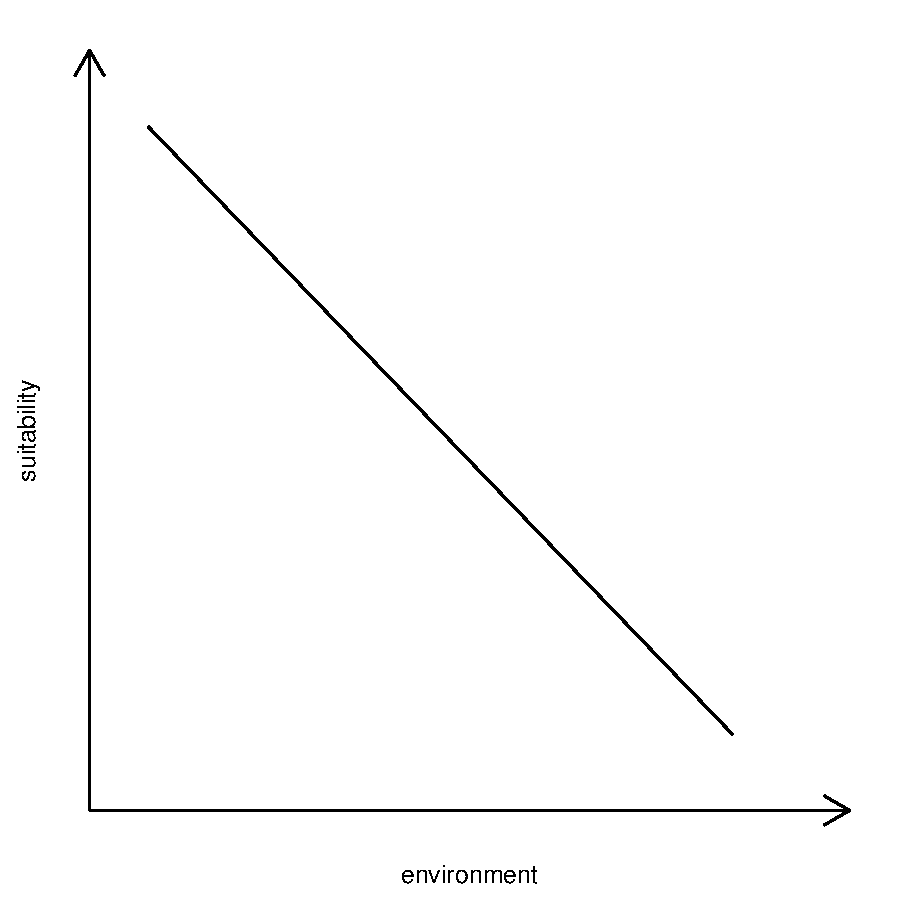
\includegraphics{sdmvspecies-linear_decreasing_function}

\subsubsection*{Truncated linear (increasing) function}
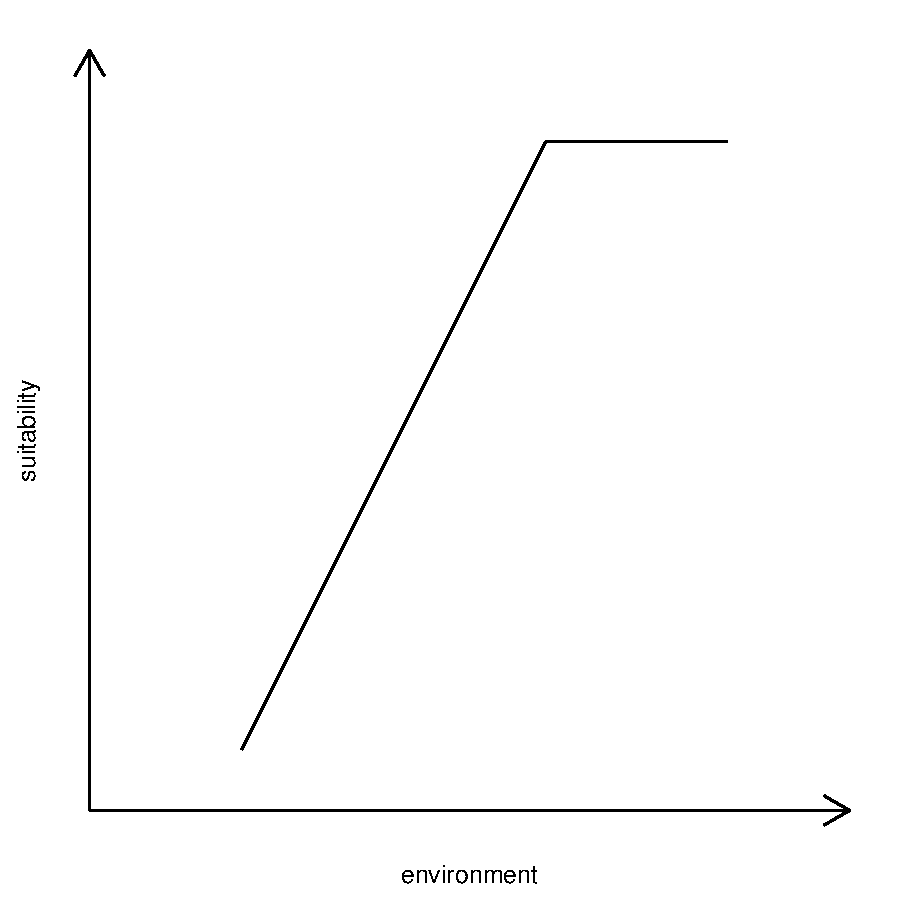
\includegraphics{sdmvspecies-truncated_linear_increasing_function}
\subsubsection*{Truncated linear (decreasing) function}
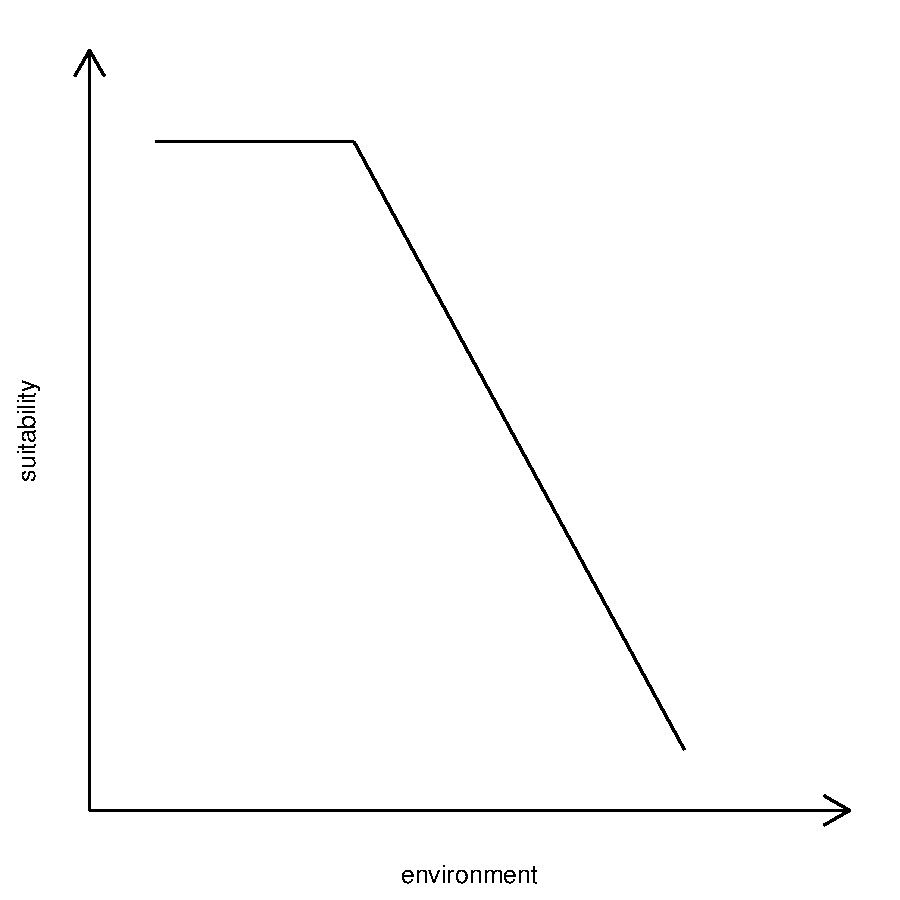
\includegraphics{sdmvspecies-truncated_linear_decrease_function}
\subsection*{Write configure code}
Response function we retruduce abover, can be use in source with certain code:
\begin{itemize}
    \item Bell-shaped function: 1
    \item Linear increase function: 2
    \item Linear decrease function: 3
    \item Truncated linear (increasing) function: 4
    \item Truncated linear (decreasing) function: 5
\end{itemize}
We see the same code used before, We change the code format for more easy to understand what we do.
\begin{Schunk}
\begin{Sinput}
> config <- list(
+     c("bio1","1",2),
+     c("bio14", "2", 2),
+     c("bio5", "3", 1),
+     c("bio11", "4", 2),
+     c("bio16", "5", 1)
+     )
\end{Sinput}
\end{Schunk}
\texttt{config} is a list in \R, it contain servel basic element like this:
\texttt{c("bio11", "4", 2)}, which \texttt{"bio11"} is the raster layer name, which always be your env name, indecate which
environment should be used, \texttt{"4"} indecate what response function we should used (Truncated linear (increasing) function), \texttt{2} is the weight.
\section*{pick mean method}
this method is first development by \citet{jimenez-valverde_threshold_2007}. Original they first use PCA (Pricipal Component Analysis) to make two main environment to present
local environment. In order to extend this method, we don't limit the environment number and the way that variable generate or pick up.
This method will consider the points fall in mean\textpm SD are suitable for virutal species occurence in one variable level, only the points fall in all variabes will conside as real occurence.
\begin{Schunk}
\begin{Sinput}
> # load the sdmvspecies library
> library("sdmvspecies")
> library("raster")
> # find package's location
> package.dir <- system.file(package="sdmvspecies")
> # let see where is our sdmvspecies is installed in
> package.dir
\end{Sinput}
\begin{Soutput}
[1] "/home/howl/R/x86_64-pc-linux-gnu-library/3.2/sdmvspecies"
\end{Soutput}
\begin{Sinput}
> # find env dir under the package's location
> env.dir <- paste(package.dir, "/external/env/", sep="")
> # let see env dir
> env.dir
\end{Sinput}
\begin{Soutput}
[1] "/home/howl/R/x86_64-pc-linux-gnu-library/3.2/sdmvspecies/external/env/"
\end{Soutput}
\begin{Sinput}
> # get the environment raster file
> file.name <- files <- c("bio1.bil", "bio12.bil", "bio7.bil", "bio5.bil")
> files <- paste(env.dir, file.name, sep="")
> # make raster stack
> env.stack <- stack(files)
> # run pick mean
> species.raster <- pickMean(env.stack)
> # plot map
> plot(species.raster)
\end{Sinput}
\end{Schunk}
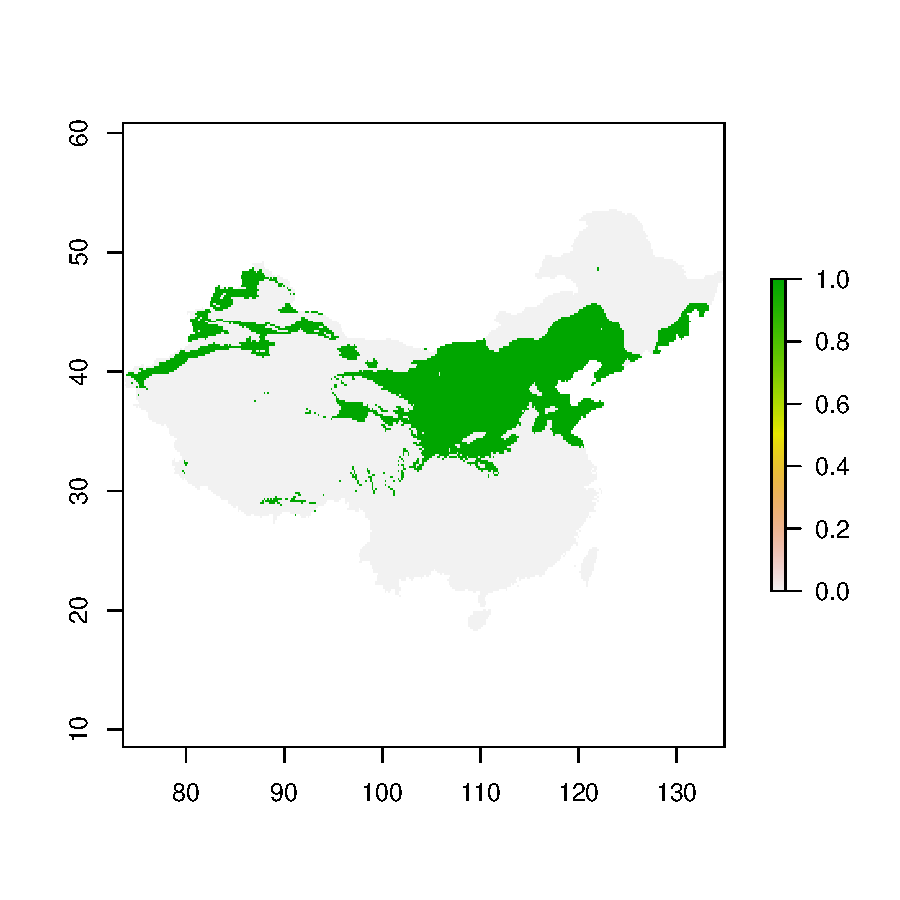
\includegraphics{sdmvspecies-pick_mean_method}
\section*{Pick median method}
This method is first development by \citet{lobo_exploring_2011}.

Original they first use PCA (Pricipal Component Analysis) to choose environment variable from candidate.
Here we don't decicus how to choose environment by using PCA or other way choose environment variable.
This method will calculate the quartiles of each variables. The points fall in the two central quartiles of variable will conside as suit for species
occurence at this variables level. The cells fall in all of variables' central quartiles will conside of species really occurence.
\begin{Schunk}
\begin{Sinput}
> # load the sdmvspecies library
> library("sdmvspecies")
> # find package's location
> package.dir <- system.file(package="sdmvspecies")
> # let see where is our sdmvspecies is installed in
> package.dir
\end{Sinput}
\begin{Soutput}
[1] "/home/howl/R/x86_64-pc-linux-gnu-library/3.2/sdmvspecies"
\end{Soutput}
\begin{Sinput}
> # find env dir under the package's location
> env.dir <- paste(package.dir, "/external/env/", sep="")
> # let see env dir
> env.dir
\end{Sinput}
\begin{Soutput}
[1] "/home/howl/R/x86_64-pc-linux-gnu-library/3.2/sdmvspecies/external/env/"
\end{Soutput}
\begin{Sinput}
> # get the environment raster file
> file.name <- files <- c("bio1.bil", "bio12.bil", "bio7.bil", "bio5.bil")
> files <- paste(env.dir, file.name, sep="")
> # make raster stack
> env.stack <- stack(files)
> # run pick mean
> species.raster <- pickMedian(env.stack)
> # plot map
> plot(species.raster)
\end{Sinput}
\end{Schunk}
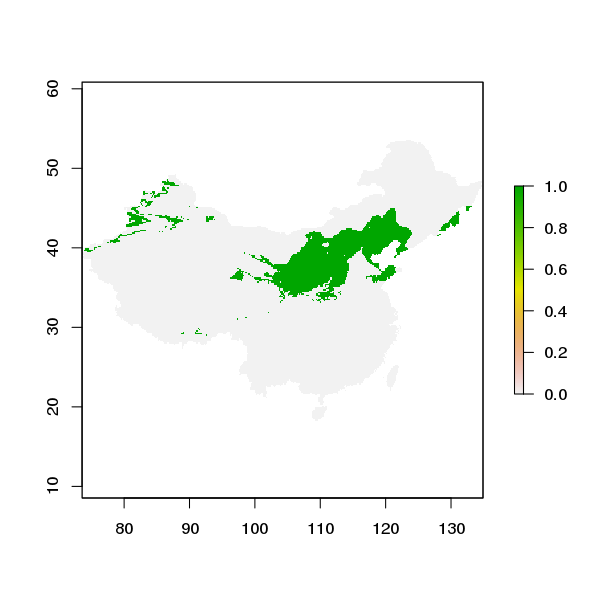
\includegraphics{sdmvspecies-pick_median_method}

\section*{Artificial Bell-shaped response method}
This method is first development by \citet{varela_environmental_2014}.
User need to specfic the mean and standard devation of normal curves (bell-shaped) for each variable. The species' overall climatic suitability was defined as the multiplication of each variables's suitability. Then User choose a threshold to make distribution map.
\begin{Schunk}
\begin{Sinput}
> # load the sdmvspecies library
> library("sdmvspecies")
> # find package's location
> package.dir <- system.file(package="sdmvspecies")
> # let see where is our sdmvspecies is installed in
> package.dir
\end{Sinput}
\begin{Soutput}
[1] "/home/howl/R/x86_64-pc-linux-gnu-library/3.2/sdmvspecies"
\end{Soutput}
\begin{Sinput}
> # find env dir under the package's location
> env.dir <- paste(package.dir, "/external/env/", sep="")
> # let see env dir
> env.dir
\end{Sinput}
\begin{Soutput}
[1] "/home/howl/R/x86_64-pc-linux-gnu-library/3.2/sdmvspecies/external/env/"
\end{Soutput}
\begin{Sinput}
> # get the environment raster file
> file.name <- files <- c("bio1.bil", "bio12.bil", "bio7.bil", "bio5.bil")
> files <- paste(env.dir, file.name, sep="")
> # make raster stack
> env.stack <- stack(files)
> # config
> config <- list(c("bio1",150, 50), c("bio12", 2000, 500), c("bio7", 400, 100), c("bio5", 300, 100))
> # run pick mean
> species.raster <- artificialBellResponse(env.stack, config)
> # plot map
> plot(species.raster)
> # species distribution map
> species.distribution.raster <- species.raster > 0.2
> # plot map
> plot(species.distribution.raster)
\end{Sinput}
\end{Schunk}
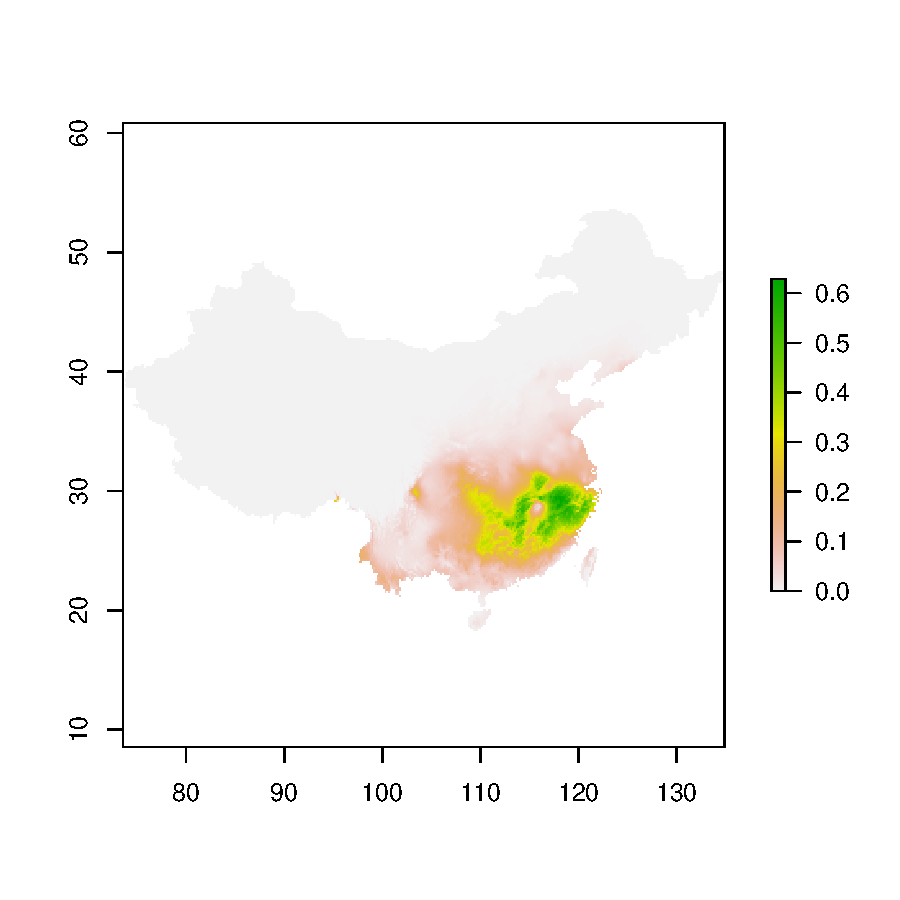
\includegraphics{sdmvspecies-artificial_bell_response_method}

The configure is a list of variable item. Each variable item contains layer name, mean and standard devation successively.

\bibliographystyle{plainnat}
\part{References}
\bibliography{bibliography}
\end{document}
